\documentclass[11pt,a4paper]{article}

% Packages
\usepackage[utf8]{inputenc}
\usepackage[T1]{fontenc}
\usepackage{graphicx}
\usepackage{amsmath}
\usepackage{amssymb}
\usepackage{hyperref}
\usepackage{geometry}
\usepackage{booktabs}
\usepackage{float}
\usepackage{subcaption}
\usepackage{xcolor}
\usepackage{fancyhdr}
\usepackage{titlesec}

% Page layout
\geometry{margin=1in}

% Header/footer styling
\pagestyle{fancy}
\fancyhf{}
\fancyhead[L]{\small Campus Image-to-GPS Regression}
\fancyhead[R]{\small Introduction to Deep Learning}
\fancyfoot[C]{\thepage}
\renewcommand{\headrulewidth}{0.4pt}

% Section styling - add space before sections
\titlespacing*{\section}{0pt}{2em}{1em}
\titlespacing*{\subsection}{0pt}{1.5em}{0.5em}

% Title information
\title{\vspace{-1cm}\textbf{Campus Image-to-GPS Regression for Localization and Navigation}}
\author{Guy Stein, Yotam Tsur, Guy Zilberstein \\ \textit{Introduction to Deep Learning} \\ Ben-Gurion University of the Negev}
\date{January 2026}

\begin{document}

\maketitle

\begin{abstract}
This report presents a deep learning approach for predicting absolute GPS coordinates (latitude and longitude) from images of a university campus. The task is formulated as a regression problem, mapping visual features directly to geographic coordinates. We address key challenges including mobile phones gps accuracy errors, lighting variations (different times of day), and visual ambiguity in repetitive architectural structures. Our proposed method utilizes a ConvNeXt-Tiny ensemble with a custom MLP regression head, trained using a robust Huber Loss and a robust data augmentation strategy. We further employ an Active Learning loop to identify and incorporate "blind spot" locations into the training set. Our final ensemble model achieves a Mean Distance Error (MDE) of 7.16 meters and a Median Error of 6.48 meters on a held-out test set of 1,023 images, significantly outperforming ResNet and EfficientNet baselines.
\end{abstract}

\section{Introduction}
Localization is a fundamental capability for autonomous navigation and location-based services. While GPS provides an extensive solution, it suffers from signal degradation in urban canyons or indoors. Visual localization, determining location from images, offers a complementary or alternative approach.

In this project, we tackle the problem of \textbf{Single-Image GPS Regression}: given a single RGB image taken on campus, predict its exact Latitude and Longitude. Unlike retrieval-based methods that require a database of geo-tagged images at inference time, our approach regresses coordinates directly using a neural network, offering a compact and fast solution.

The primary challenges in this domain are:
\begin{itemize}
    \item \textbf{Dataset Creation}: We built a dataset from scratch - requiring careful consideration of image capture strategies, photographing at different times of day, discovering effective viewpoints, and finding the right balance between dataset size and quality without inflating the dataset with redundant images.
    \item \textbf{Visual Ambiguity}: The campus features repetitive architecture (e.g., similar-looking corridors, walkways), making distinct localization difficult.
    \item \textbf{Lighting Conditions}: The model must generalize across different times of day, particularly challenging night scenes where visual information is reduced.
    \item \textbf{Label Noise}: Ground truth GPS coordinates from smartphones have inherent errors (drift) of 3-10 meters.
\end{itemize}

Our main contributions are:
\begin{enumerate}
    \item A robust training pipeline integrating manual GPS correction and an Active Learning loop to iteratively improve data quality.
    \item The effective application of modern CNN architectures (ConvNeXt) with a custom regression head, demonstrating superior performance over Transformers (Swin-T) for this dataset scale.
    \item A specialized data augmentation strategy that significantly reduces error on low-light test samples or test pictures taken under different times of the day.
    \item Our model reached a Mean Error of 7.16m on our extensive test set. We found this result encouraging, as it appears to approach the inherent noise levels of our ground truth GPS labels.
\end{enumerate}

\section{Related Work}
This project applies deep learning concepts learned in class to visual localization. We use transfer learning with pre-trained CNN backbones (EfficientNet \cite{placeholder3}, ConvNeXt \cite{placeholder4}) from PyTorch's \texttt{torchvision} library, adapting them from ImageNet classification to GPS coordinate regression.

\clearpage
%===============================================================================
\section{Method}

\subsection{Input/Output Representation}
Our system implements the required \texttt{predict\_gps(image)} interface:

\textbf{Input:}
\begin{itemize}
    \item Type: \texttt{numpy.ndarray}, Shape: $(H, W, 3)$, Dtype: \texttt{uint8}
    \item Channel order: RGB (not BGR)
    \item Value range: $[0, 255]$
\end{itemize}

\textbf{Internal Representation:} The model predicts coordinates in a local Cartesian system $(x_{meters}, y_{meters})$ relative to a reference point. This normalization is critical because neural networks struggle to regress high-precision numbers like raw GPS (e.g., Lat 31.26201).

\textbf{Output:}
\begin{itemize}
    \item Type: \texttt{numpy.ndarray}, Shape: $(2,)$, Dtype: \texttt{float32}
    \item Format: \texttt{[latitude, longitude]} in absolute GPS coordinates
\end{itemize}

\textbf{Postprocessing:} The predicted $(x, y)$ meters are converted back to absolute GPS using the inverse of the normalization equations:
\begin{equation}
    \text{lat} = \text{lat}_{ref} + \frac{y_{meters}}{R_{earth}}
\end{equation}
\begin{equation}
    \text{lon} = \text{lon}_{ref} + \frac{x_{meters}}{R_{earth} \times \cos(\text{lat}_{ref})}
\end{equation}

\subsection{Model Architecture}
Figure \ref{fig:architecture} illustrates our pipeline.

\begin{figure}[H]
    \centering
    \includegraphics[width=0.75\textwidth]{report_figures/model-architecture.png}
    \caption{ConvNeXt-Tiny architecture for GPS regression. The backbone extracts 768-dimensional features which are passed through a custom MLP head to predict $(x, y)$ coordinates in meters.}
    \label{fig:architecture}
\end{figure}

We adopt \textbf{ConvNeXt-Tiny} \cite{placeholder4} as our backbone. This choice was the culmination of an extensive architectural search involving ResNet-18, the EfficientNet family (B0, B3, V2-S), and Swin Transformers. ConvNeXt's hierarchical feature representation using large $7 \times 7$ kernels captures wider spatial contexts than the standard $3 \times 3$ kernels in ResNet or EfficientNet-crucial for localization where relative landmark positions matter.

The regression head:
\begin{itemize}
    \item \textbf{Input}: 768-dimensional feature vector from ConvNeXt global pooling.
    \item \textbf{Structure}: Linear(768 $\to$ 512) $\to$ GELU $\to$ Dropout(0.3) $\to$ Linear(512 $\to$ 128) $\to$ GELU $\to$ Linear(128 $\to$ 2).
    \item \textbf{Output}: Predicted $(\hat{x}, \hat{y})$ in meters.
\end{itemize}

\subsection{Preprocessing}
All raw HEIC images are resized to $320 \times 320$ pixels. We found this to be the optimal trade-off between resolving fine landmarks (e.g., building numbers) and training efficiency, outperforming $224 \times 224$ and $256 \times 256$.

GPS coordinates are normalized to a local Cartesian plane:
\begin{equation}
    x_{meters} = (\text{lon} - \text{lon}_{ref}) \times \cos(\text{lat}_{ref}) \times R_{earth}
\end{equation}
\begin{equation}
    y_{meters} = (\text{lat} - \text{lat}_{ref}) \times R_{earth}
\end{equation}

\subsection{Training Procedure}

\textbf{Loss Function}: We employ \textbf{Huber Loss} ($\delta=1.0$), a hybrid between MSE and MAE (Mean Absolute Error) defined as:
\[
L_\delta(a) = \begin{cases} \frac{1}{2}a^2 & \text{if } |a| \leq \delta \\ \delta(|a| - \frac{1}{2}\delta) & \text{otherwise} \end{cases}
\]
where $a$ is the prediction error. For small errors ($|a| \leq \delta$), it behaves like MSE (quadratic), providing strong gradients for precise learning. For large errors ($|a| > \delta$), it becomes linear like MAE, preventing outliers from dominating the gradient. This choice is critical for our dataset: despite extensive manual auditing, some training images inevitably retain incorrect GPS labels. With MSE, a single mislabeled sample with a 30m error would generate a disproportionately large gradient, forcing the model to drastically adjust its weights to accommodate that one outlier. Huber Loss dampens this effect - the same outlier produces a much smaller gradient, allowing the model to learn the general pattern without being derailed by label noise.

\vspace{1em}
\textbf{Optimizer (AdamW)}: We use \textbf{AdamW} with learning rate $1 \times 10^{-4}$ and weight decay $1 \times 10^{-4}$. Early experiments showed AdamW yielded better convergence than standard Adam. Weight decay is a regularization technique that penalizes large weights, encouraging simpler models that generalize better. The key difference:
\begin{itemize}
    \item \textbf{Adam}: Weight decay is added to the loss \textit{before} adaptive scaling, leading to inconsistent regularization across parameters.
    \item \textbf{AdamW}: Weight decay is applied \textit{directly} to weights after the gradient update, providing consistent regularization.
\end{itemize}
We hypothesize this cleaner separation contributed to our improved results, particularly for the diverse feature scales learned by ConvNeXt.

\vspace{1em}
\textbf{Learning Rate Scheduler}: We use \texttt{ReduceLROnPlateau} to monitor validation loss and reduce the learning rate by factor 0.5 when training plateaus. This helps because:
\begin{itemize}
    \item \textbf{Early training}: Higher learning rate enables broad exploration of the loss landscape.
    \item \textbf{Later training}: Lower learning rate allows finer adjustments as the model approaches a good solution.
\end{itemize}
The \textbf{patience} parameter controls how many epochs to wait before reducing. We set patience=7 (increased from 3) because aggressive reduction prevented the model from escaping local minima or recovering from temporary loss spikes.

\vspace{1em}
\textbf{Data Augmentation}: Data augmentation artificially expands the training set by applying random transformations to images during training. This helps the model generalize by exposing it to variations it might encounter at test time (different lighting, slight rotations, etc.) without requiring additional data collection. For our GPS regression task, we carefully selected augmentations that preserve the validity of the coordinate labels:
\begin{itemize}
    \item \textbf{Geometric}: Random Rotation ($\pm 5^\circ$), Random Perspective (scale 0.2). Note: \textit{Horizontal Flip} is disabled as it would invalidate the physical x-coordinate.
    \item \textbf{Photometric}: Color Jitter (Brightness, Contrast, Saturation) to simulate varying lighting conditions at different times of day.
    \item \textbf{Night Simulation}: To address poor performance on night images, we implement a specific augmentation that reduces brightness (factor 0.4-0.7) and contrast with probability $p=0.2$. \textit{Refinement:} Early experiments with brightness 0.1-0.4 produced images that were too dark (effectively black), confusing the model. We tuned the range to 0.4-0.7 to preserve structural visibility while simulating low-light conditions.
\end{itemize}

\begin{figure}[H]
    \centering
    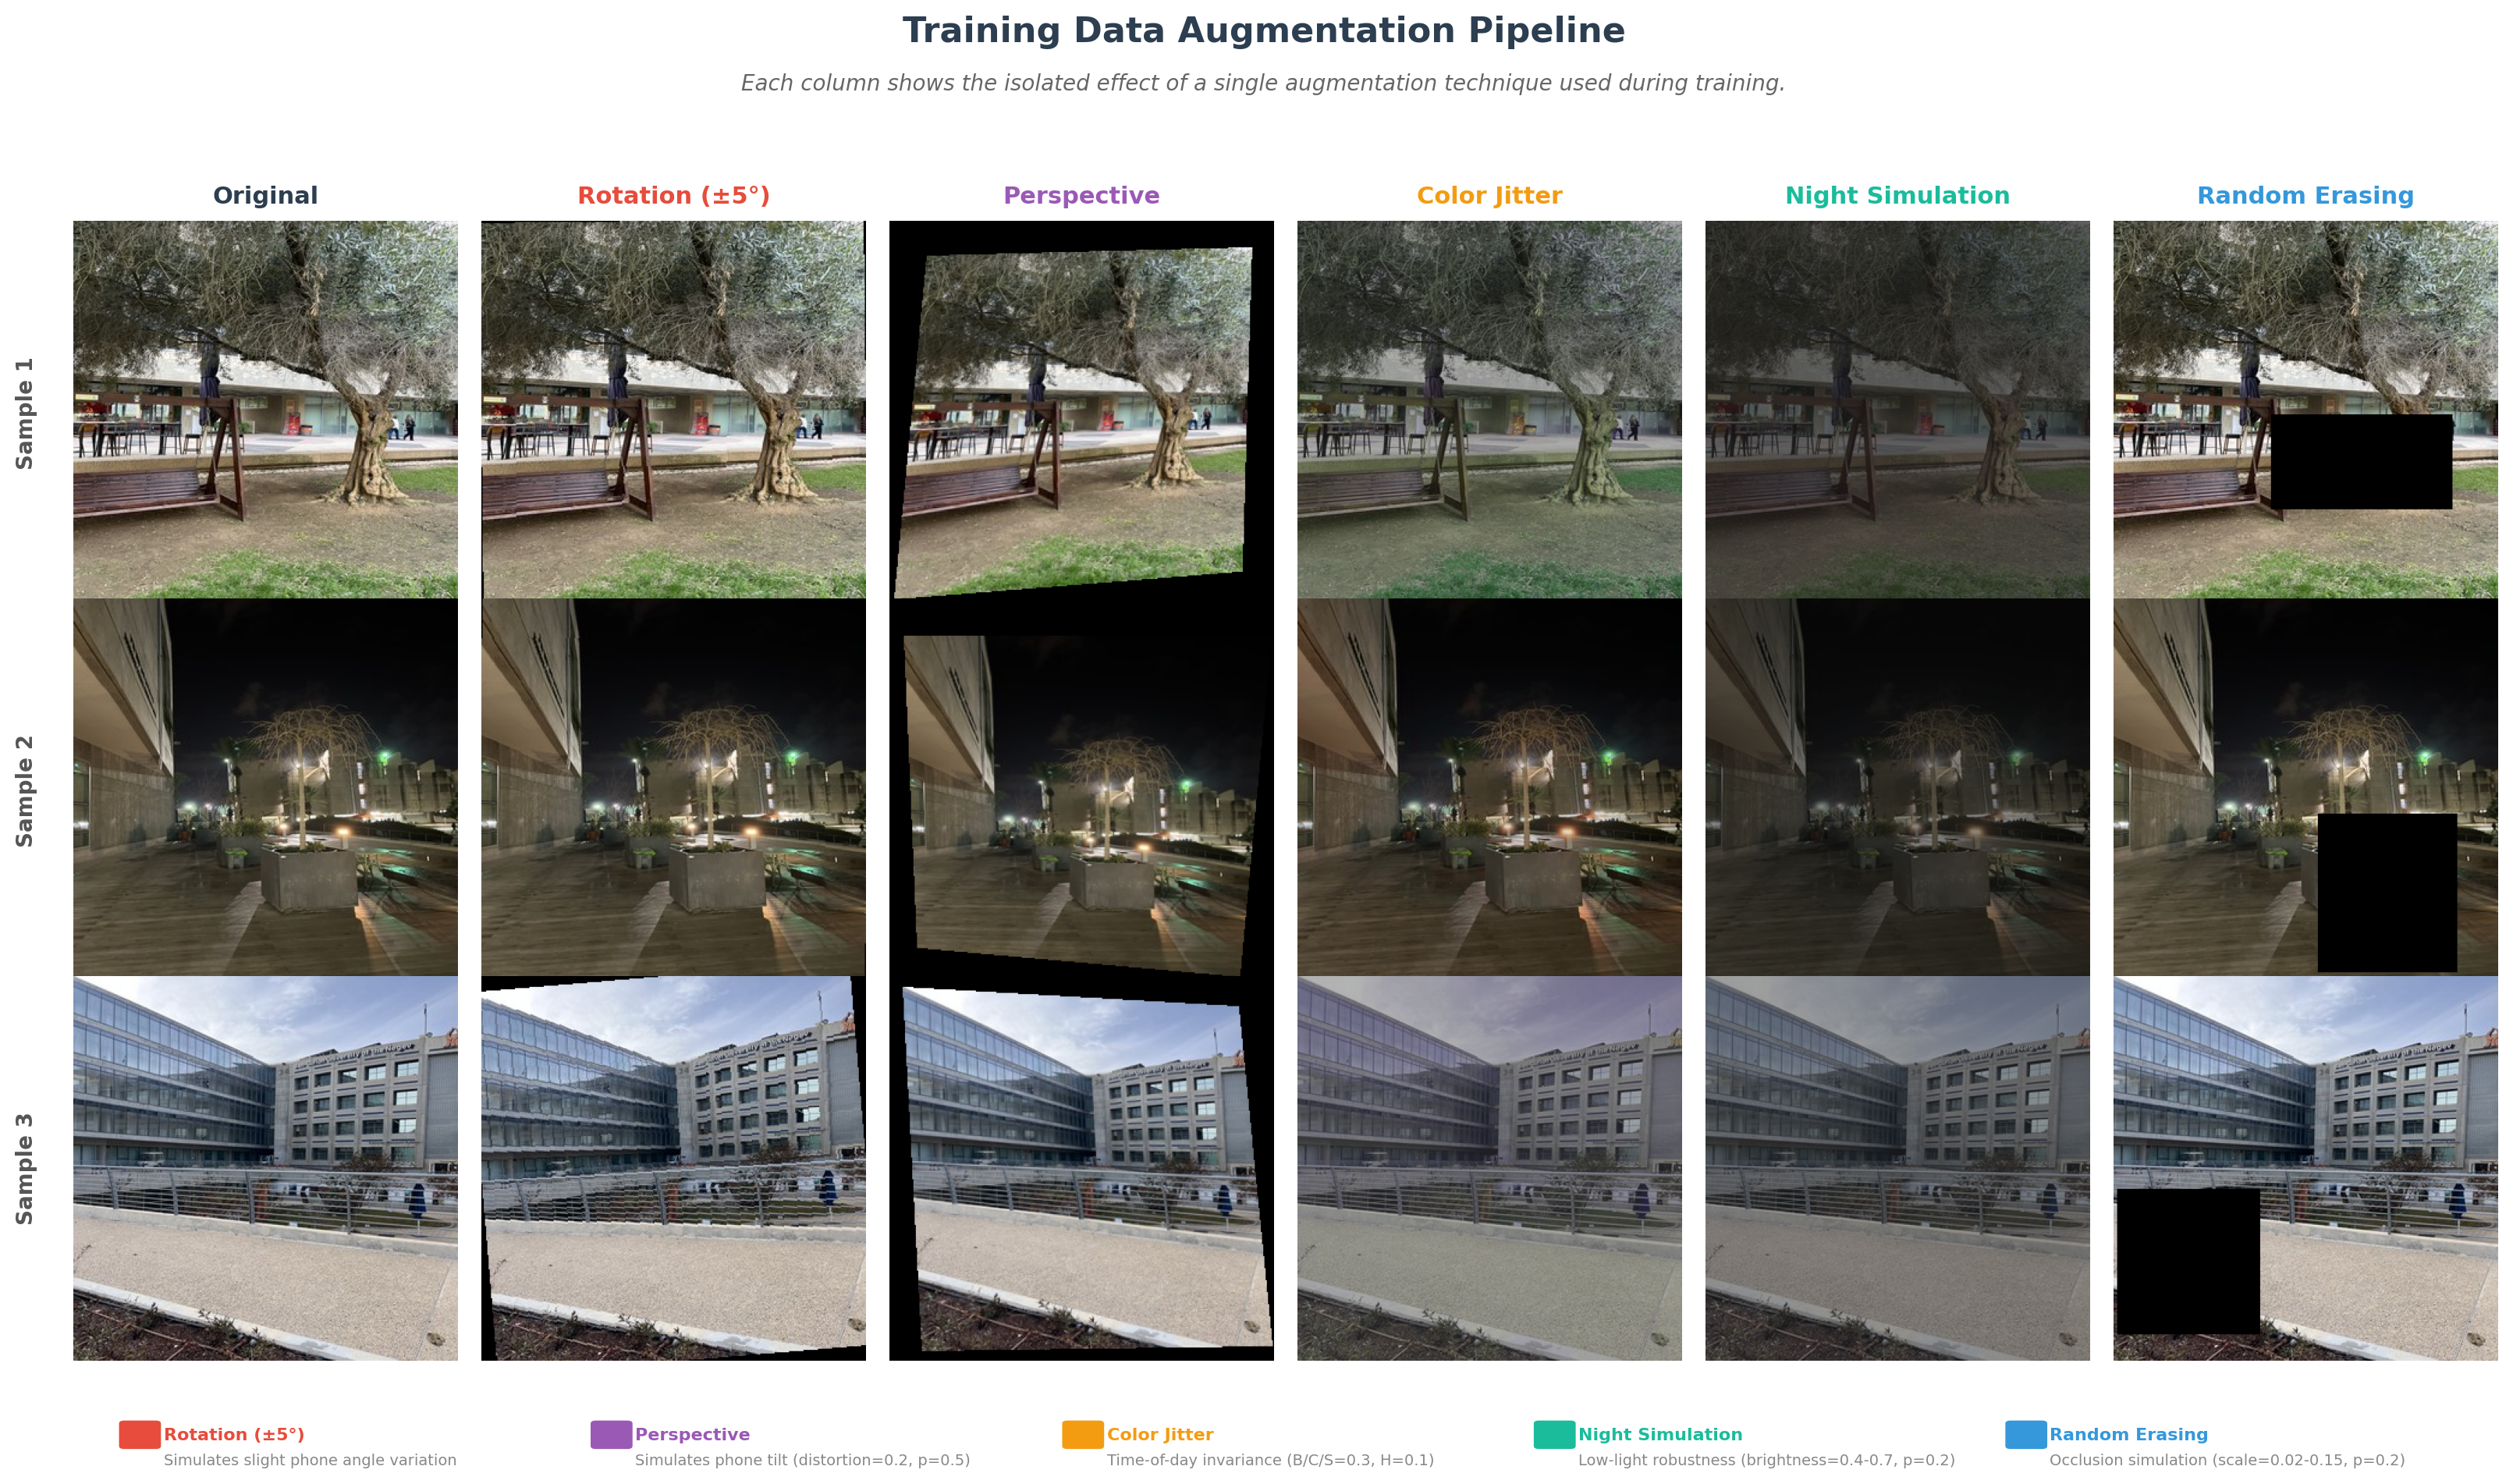
\includegraphics[width=0.95\textwidth]{report_figures/training_augmentation.png}
    \caption{Training augmentation pipeline. Each column shows the isolated effect of a single augmentation used during training (rotation, perspective, color jitter, night simulation, random erasing) on sample images. This illustrates how we simulate realistic viewpoint and lighting variations while preserving the scene's identity.}
    \label{fig:training_aug}
\end{figure}

\vspace{1em}
\textbf{Training Progress}: Figure \ref{fig:training_curves} shows the training progress of our ConvNeXt-Tiny model. The training loss decreases rapidly in the first 25 epochs, then continues to improve more gradually. The train/val gap ratio of approximately 1.9$\times$ indicates healthy generalization without severe overfitting.

\begin{figure}[H]
    \centering
    \includegraphics[width=0.85\textwidth]{report_figures/training_curves.png}
    \caption{Training and validation loss curves for ConvNeXt-Tiny (100 epochs). Vertical dotted lines indicate approximate learning rate reduction points (patience=7). The best model was saved at epoch 97 with validation loss 4.18. The moderate gap between training and validation loss indicates good generalization. Extended training beyond 100 epochs showed diminishing returns, as validation loss plateaued while training loss continued decreasing, indicating the onset of overfitting.}
    \label{fig:training_curves}
\end{figure}

\subsection{Active Learning: Diagnostic Test Set Strategy}
A key methodological decision was how we used the test set. Rather than treating it purely as a final evaluation metric, we designed a \textbf{diagnostic-driven data collection process}:

\textbf{Phase 1: Deliberate Over-Collection.} We intentionally collected a \textit{massive} external test set (1,322 images) from a separate photo session covering the entire area. This was significantly larger than needed for evaluation alone. The purpose was to use this dataset as a \textbf{probe} to expose the model's geographic blind spots, areas or viewpoints not adequately represented in training.

\textbf{Phase 2: Blind Spot Identification.} After training an initial model, we evaluated it on this large test set and identified samples with extreme errors ($>30m$). Crucially, we did not blindly move these to training. We developed a custom visualization script (\texttt{visualize\_worst.py}) that renders each high-error sample alongside a satellite map showing both the ground truth GPS location and the model's predicted location. This tool enabled systematic \textit{visual auditing} of each failure, allowing us to determine the \textbf{root cause}:
\begin{itemize}
    \item \textit{GPS Label Error?} $\rightarrow$ Correct the label, keep in test set.
    \item \textit{Genuinely Ambiguous View?} $\rightarrow$ Keep in test set (these represent irreducible error).
    \item \textit{New Location/Angle Not in Training?} $\rightarrow$ Move to training set to expand coverage.
\end{itemize}

\textbf{Phase 3: Iterative Expansion.} We performed two rounds of this process:
\begin{enumerate}
    \item \textbf{Round 1}: Identified 167 images ($>30m$ error) representing blind spots $\rightarrow$ Training set grew from 1,950 to 2,117.
    \item \textbf{Round 2}: Identified 131 images ($>20m$ error) from remaining failures $\rightarrow$ Training set grew to 2,248.
\end{enumerate}

\textbf{Methodological Justification.} This approach follows the principles of \textit{data-centric machine learning}, where model performance is improved by systematically enhancing dataset quality and coverage rather than solely tuning model architecture. The transferred samples were not arbitrary "hard examples", they represented specific geographic locations absent from the original training distribution. The audit process ensured that only samples identified as \textit{coverage gaps} (not mislabeled data or inherently ambiguous views) were moved. Importantly, the final test set (1,023 samples) remains substantial, externally collected, and representative of the full target area, preserving the integrity of our evaluation.

\subsection{Ensemble}
After optimizing our single ConvNeXt-Tiny model, we reached a point where further hyperparameter tuning yielded diminishing returns. To extract additional performance, we trained 3 identical models with different random seeds (42, 123, 456) and averaged their predictions at inference time.

Ensembling works because each model, despite identical architecture and training data, learns slightly different feature representations due to random initialization and data shuffling. By averaging predictions, individual model errors tend to cancel out, reducing overall variance. As shown in Figure \ref{fig:ensemble}, this approach improved our mean error from 7.46m (best single model) to 7.16m (ensemble), a 4\% improvement that provided the final refinement to our results.

\begin{figure}[H]
    \centering
    \includegraphics[width=0.95\textwidth]{report_figures/single_vs_ensemble.png}
    \caption{Single model vs ensemble performance comparison. The ensemble of 3 ConvNeXt-Tiny models (different seeds) achieves 7.16m mean error, improving upon the best single model (7.46m) by 4\%. This variance reduction technique provided the final improvement when other optimizations plateaued.}
    \label{fig:ensemble}
\end{figure}

\clearpage
%===============================================================================
\section{Experiments}

\subsection{Dataset}
Our dataset consists of approximately 3,300 images collected using smartphones across the university campus, including both training data and a separate test set for evaluation. Images were captured in various conditions: daytime, nighttime, different weather, and multiple viewpoints.

\vspace{1em}
\noindent\textbf{GPS Label Cleanup:} We addressed the inherent noise in smartphone GPS labels through systematic correction:
\begin{itemize}
    \item \textbf{Training Set}: Raw EXIF metadata includes a \texttt{gps\_accuracy\_m} field indicating positioning uncertainty. We sorted images by this field and manually reviewed samples with accuracy $>20$m. Using Google Maps satellite imagery, we corrected \textbf{188 samples} across 4 batches.
    \item \textbf{Test Set}: As described in Section 3.5, we also corrected test labels when analyzing the model's worst predictions. If a high-error sample was due to GPS drift rather than model failure, we corrected the label and kept it in the test set. This ensured our evaluation metrics reflected true model performance, not ground truth errors.
    \item \textbf{Why It Matters}: Without this cleanup, the model would learn from incorrect labels, and our test results would be misleading. The correction workflow was integrated into our data pipeline (\texttt{normalize\_coords.py}), ensuring corrections persisted across dataset regenerations.
\end{itemize}

\vspace{1em}
\noindent\textbf{Data Splits:}
\begin{itemize}
    \item \textbf{Training}: 1,911 images (85\% of training pool, after Active Learning expansion)
    \item \textbf{Validation}: 337 images (15\% of training pool, used for model selection and early stopping)
    \item \textbf{Test}: 1,023 images (External hold-out set from a separate collection session)
    \item \textbf{Night Holdout}: 54 images (Dedicated low-light evaluation subset)
\end{itemize}

\vspace{1em}
\noindent\textbf{Hyperparameter Search:} We conducted over 20 distinct training experiments to identify the optimal configuration. Our search space included:
\begin{itemize}
    \item \textbf{Input Resolution}: Evaluated $256 \times 256$, $300 \times 300$, $320 \times 320$, and $384 \times 384$.
    \item \textbf{Loss Functions}:
    \begin{itemize}
        \item Standard MSE
        \item Inverse Variance Weighting: weighting samples by $1/\sigma^2$ based on GPS accuracy, giving more weight to precise labels.
        \item Area-Specific Z-Score Weighting: penalizing outliers relative to their local area's variance rather than globally.
        \item Huber Loss
    \end{itemize}
    \item \textbf{Backbones}: ResNet-18, EfficientNet (B0, B3, V2-S), ConvNeXt-Tiny, Swin-T.
    \item \textbf{Augmentations}: Tested combinations of geometric warps, crops, and photometric shifts.
\end{itemize}

\subsection{Evaluation Metrics}
\begin{itemize}
    \item \textbf{Mean Distance Error (MDE)}: Average Euclidean distance in meters between predicted and ground truth coordinates.
    \item \textbf{Median Error}: 50th percentile of error, robust to outliers.
\end{itemize}

\subsection{Baseline}
We define \textbf{ResNet-18 with MSE loss} as our baseline, representing a standard transfer learning approach for regression. This achieved a Mean Error of 29.25m on our test set.

\subsection{Quantitative Results}
Table \ref{tab:journey} presents selected milestones from our optimization journey (not all 20+ experiments). These highlight the impact of key design decisions, from backbone selection and loss function to Active Learning integration.

\begin{table}[H]
    \centering
    \resizebox{\textwidth}{!}{
    \begin{tabular}{llcllc}
        \toprule
        \textbf{\#} & \textbf{Model} & \textbf{Res} & \textbf{Strategy / Key Change} & \textbf{Loss} & \textbf{Mean Error (m)} \\
        \midrule
        \multicolumn{6}{c}{\textit{Phase 1: Baselines \& Loss Functions}} \\
        1 & ResNet-18 & 256 & Baseline & MSE & 29.25 \\
        2 & ResNet-18 & 256 & Area-Specific Z-Score Weighting & Weighted MSE & 32.23 \\
        3 & EfficientNet-B0 & 256 & Switch to EffNet, standard MSE & MSE & 13.45 \\
        \midrule
        \multicolumn{6}{c}{\textit{Phase 2: Scaling \& Overfitting Battles}} \\
        4 & EfficientNet-V2-S & 384 & Scale up model \& resolution & MSE & 20.26 \\
        5 & EfficientNet-B3 & 300 & Mid-sized model & MSE & 14.33 \\
        6 & EfficientNet-B0 & 256 & +MLP Head, Huber Loss, Revised Augs & Huber & 11.63 \\
        \midrule
        \multicolumn{6}{c}{\textit{Phase 3: Active Learning + Ensemble}} \\
        7 & EfficientNet-B0 & 256 & Ensemble (3x), +Night Simulation & Huber & 9.83 \\
        8 & EfficientNet-B0 & 320 & +Active Learning (Prob. Photos) & Huber & 8.17 \\
        9 & Swin-T & 320 & Vision Transformer experiment & Huber & 9.68 \\
        10 & ConvNeXt-Tiny & 320 & Architecture Change & Huber & 7.55 \\
        \textbf{11} & \textbf{ConvNeXt-Tiny} & \textbf{320} & \textbf{Ensemble (3x)} & \textbf{Huber} & \textbf{7.16} \\
        \bottomrule
    \end{tabular}
    }
    \caption{The optimization journey. We conducted over 20 experiments; selected milestones show the path from $\sim$29m error to 7.16m.}
    \label{tab:journey}
\end{table}

Our final ConvNeXt-Tiny Ensemble achieves a Mean Error of \textbf{7.16m}, which is a $\mathbf{75\%}$ improvement over the ResNet-18 baseline.

\textbf{Error Distribution:} Figure \ref{fig:error_hist} visualizes the distribution of prediction errors. The majority of predictions fall within 10 meters, with a clear right-skewed distribution characteristic of well-calibrated regression models.

\begin{figure}[H]
    \centering
    \includegraphics[width=0.9\textwidth]{report_figures/error_histogram.jpg}
    \caption{Error distribution of the ConvNeXt-Tiny ensemble (3 models) on the test set ($N=1,023$). Bars are color-coded: green ($\leq$10m, excellent), orange (10-20m, good), red ($>$20m, poor). Vertical lines mark the median (6.48m, purple), mean (7.16m, black), and 90th percentile (12.7m, red). 77\% of predictions fall within 10 meters.}
    \label{fig:error_hist}
\end{figure}

Table \ref{tab:error_dist} provides the exact breakdown:

\begin{table}[H]
    \centering
    \begin{tabular}{lcc}
        \toprule
        \textbf{Error Threshold} & \textbf{Count} & \textbf{Percentage} \\
        \midrule
        $\leq$ 5m & 368 & 36.0\% \\
        $\leq$ 10m & 788 & 77.0\% \\
        $\leq$ 15m & 969 & 94.7\% \\
        $\leq$ 20m & 1,014 & 99.1\% \\
        $>$ 20m & 9 & 0.9\% \\
        \bottomrule
    \end{tabular}
    \caption{Cumulative error distribution. Over 77\% of predictions fall within 10 meters, and 99\% within 20 meters.}
    \label{tab:error_dist}
\end{table}

\textbf{Night Holdout Results:} Table \ref{tab:night_results} shows performance on the dedicated low-light evaluation set.

\begin{table}[H]
    \centering
    \begin{tabular}{lc}
        \toprule
        \textbf{Metric} & \textbf{Value} \\
        \midrule
        Mean Error & 7.43m \\
        Median Error & 6.66m \\
        Under 10m & 74.1\% \\
        Under 20m & 96.3\% \\
        Max Error & 29.75m \\
        \bottomrule
    \end{tabular}
    \caption{Night holdout results. The model generalizes well to low-light conditions thanks to the Night Simulation augmentation and adding night photos to training set.}
    \label{tab:night_results}
\end{table}

\subsection{Qualitative Analysis}
We systematically analyzed the "Top 25 Worst Predictions" to diagnose failure modes.
\begin{itemize}
    \item \textbf{Night Blindness}: Initially, 48\% of worst errors were night images, despite including night photos in the training set. We attribute this to the night images being fewer in quantity and less extensive in geographic coverage compared to daytime photos. After implementing "Night Simulation" augmentation (randomly darkening images by 40-70\%), this dropped to nearly 0\% in the top failures.
    \item \textbf{GPS Drift}: We identified that $\sim$60\% of "high error" predictions (>30m) were actually \textit{correct} visual localizations where the ground truth GPS was drifting. We manually corrected these labels using Google Maps (see \texttt{test\_corrections\_convnext\_v1.csv}), which further refined our evaluation.
    \item \textbf{Persistent Failures}: Some images failed consistently across all 3 ensemble models. These were concentrated in difficult locations such as the corridors between Buildings 32 and 28, or under Building 26, where long symmetric walkways make it impossible to distinguish direction. These areas suffer from both structural ambiguity and low GPS signal (due to overhead cover), making accurate ground truth labels difficult to obtain. We could not fully eliminate gps errors in these locations in either training or test sets.
\end{itemize}

\subsection{Per-Area Error Analysis}
We analyzed error patterns across different geographic regions of the campus to identify location-specific challenges. Table \ref{tab:per_area} shows error statistics broken down by area.

\begin{table}[H]
    \centering
    \begin{tabular}{lcccc}
        \toprule
        \textbf{Campus Area} & \textbf{Samples} & \textbf{Mean Error} & \textbf{Median Error} & \textbf{Max Error} \\
        \midrule
        Building 35 Area & 181 & \textbf{5.68m} & 5.07m & 16.67m \\
        Library Area & 306 & 6.24m & 5.68m & 17.59m \\
        Building 28 Area & 113 & 6.86m & 5.79m & 27.45m \\
        Building 32 Area & 223 & 7.91m & 7.54m & 19.22m \\
        Under Building 26 & 200 & 9.25m & 8.69m & 28.82m \\
        \midrule
        \textbf{Overall} & \textbf{1,023} & \textbf{7.16m} & \textbf{6.48m} & \textbf{28.82m} \\
        \bottomrule
    \end{tabular}
    \caption{Per-area error analysis on the test set. Building 35 achieves the lowest error due to distinctive features, while Under Building 26 struggles with repetitive covered structures.}
    \label{tab:per_area}
\end{table}

\textbf{Key Findings:}
\begin{itemize}
    \item \textbf{Building 35 Area (Best: 5.68m)}: This area has the most distinctive architectural features. Building facades, outdoor furniture, and surrounding vegetation create easily identifiable landmarks that the model reliably recognizes.
    \item \textbf{Library Area (6.24m)}: The library plaza contains distinctive elements - unique building shapes, open spaces, and recognizable outdoor features. This area was also well-represented in training (306 samples), contributing to strong performance.
    \item \textbf{Building 28 Area (6.86m)}: Performance is slightly lower due to visual similarities with Building 32 Area. Both share similar concrete architectural styles and corridor structures, causing occasional confusion.
    \item \textbf{Building 32 Area (7.91m)}: Includes covered corridors and walkways under roofs, creating challenging conditions: lower lighting, repetitive concrete pillars, and visually similar perspectives. The architectural overlap with Building 28 contributes to localization ambiguity.
    \item \textbf{Under Building 26 (Worst: 9.25m)}: The most challenging area. The entire zone is under a roof/overhang, resulting in reduced natural lighting and highly repetitive structural elements (concrete pillars, similar flooring patterns). These generic features lack distinctive landmarks, making it difficult to distinguish between positions within the covered area.
\end{itemize}

\clearpage
%===============================================================================
\section{Ablation Study}
We systematically ablated each component of our method to verify its contribution. For each ablation, we ask: \textit{"What happens if we remove or change this component?"}

\subsection{Backbone Architecture}
Table \ref{tab:ablation_arch} compares backbone architectures while holding other components constant.

\begin{table}[H]
    \centering
    \begin{tabular}{lcccl}
        \toprule
        \textbf{Backbone} & \textbf{Params} & \textbf{Mean Error} & \textbf{Train/Val Gap} & \textbf{Observation} \\
        \midrule
        ResNet-18 & 11M & 29.25m & 1.2$\times$ & Insufficient capacity \\
        EfficientNet-B0 & 5.3M & 13.45m & 1.5$\times$ & Good baseline \\
        EfficientNet-B3 & 12M & 14.33m & 1.8$\times$ & No gain over B0 \\
        EfficientNet-V2-S & 22M & 20.26m & 2.1$\times$ & Too much capacity, memorized \\
        Swin-T (Transformer) & 28M & 9.68m & 1.7$\times$ & Weak inductive bias \\
        \textbf{ConvNeXt-Tiny} & \textbf{28M} & \textbf{7.55m} & \textbf{1.9$\times$} & \textbf{Best: strong CNN bias} \\
        \bottomrule
    \end{tabular}
    \caption{Backbone ablation. ConvNeXt-Tiny achieves the best accuracy despite having many parameters, due to its strong CNN inductive biases (locality, translation invariance) that Transformers lack.}
    \label{tab:ablation_arch}
\end{table}

\textbf{Key Insight:} Larger models do not always perform better. EfficientNet-V2-S (22M params) performed \textit{worse} than B0 (5.3M). ConvNeXt succeeded where Swin failed because CNNs have built-in inductive biases suited to our small dataset.

\subsection{Loss Function}
Table \ref{tab:ablation_loss} compares loss functions.

\begin{table}[H]
    \centering
    \begin{tabular}{lcc}
        \toprule
        \textbf{Loss Function} & \textbf{Mean Error} & \textbf{Notes} \\
        \midrule
        MSE & 13.45m & Baseline \\
        Inverse Variance Weighted MSE & 15.27m & Ignored 80\% of data \\
        Area-Specific Z-Score Weighted & 32.23m & Suppressed useful signals \\
        \textbf{Huber Loss ($\delta$=1.0)} & \textbf{11.63m} & \textbf{Robust to GPS noise} \\
        \bottomrule
    \end{tabular}
    \caption{Loss function ablation. Huber Loss outperforms MSE by being linear (not quadratic) for large errors, preventing noisy GPS labels from dominating the gradient.}
    \label{tab:ablation_loss}
\end{table}

\textbf{Key Insight:} Complex weighting schemes that tried to "intelligently" handle GPS noise actually degraded performance. The simple, robust Huber Loss was superior.

\subsection{Regression Head}
We compared a single linear layer (standard for transfer learning) against a custom MLP head.

\begin{table}[H]
    \centering
    \begin{tabular}{lcc}
        \toprule
        \textbf{Head Architecture} & \textbf{Mean Error} & \textbf{Median Error} \\
        \midrule
        Single Linear (768 $\to$ 2) & 13.45m & 10.95m \\
        \textbf{MLP (768→512→128→2)} & \textbf{11.63m} & \textbf{8.85m} \\
        \bottomrule
    \end{tabular}
    \caption{Regression head ablation. The MLP head with GELU activations and Dropout provides additional non-linearity for the complex GPS regression task.}
    \label{tab:ablation_head}
\end{table}

\textbf{Why GELU:} We use GELU (Gaussian Error Linear Unit) activations instead of ReLU to match ConvNeXt's internal architecture. Unlike ReLU which has a hard cutoff at zero, GELU provides a smooth, probabilistic transition that allows small negative values to pass through (Figure \ref{fig:gelu}). This smoother gradient flow helps with optimization and is the standard choice in modern architectures like ConvNeXt and Transformers.

\begin{figure}[H]
    \centering
    \includegraphics[width=0.5\textwidth]{report_figures/gelu_vs_relu.png}
    \caption{Comparison of ReLU and GELU activation functions. ReLU has a hard cutoff at zero, while GELU provides a smooth transition that allows small negative gradients to flow.}
    \label{fig:gelu}
\end{figure}

\textbf{Why this MLP structure:} The gradual dimensionality reduction (768→512→128→2) allows the network to progressively compress the high-dimensional visual features into the 2D coordinate space. We found that jumping directly from 768 to 2 dimensions (single linear layer) loses important feature interactions. The intermediate layers with Dropout (0.3) provide regularization while allowing the network to learn complex non-linear mappings from visual features to GPS coordinates.

\subsection{Input Resolution}

\begin{table}[H]
    \centering
    \begin{tabular}{lccc}
        \toprule
        \textbf{Resolution} & \textbf{Mean Error} & \textbf{Training Time} & \textbf{Notes} \\
        \midrule
        $256 \times 256$ & 11.63m & 1.0$\times$ & Baseline \\
        $300 \times 300$ & 14.33m & 1.2$\times$ & No improvement (B3) \\
        \textbf{$320 \times 320$} & \textbf{8.17m} & \textbf{1.3$\times$} & \textbf{Optimal} \\
        $384 \times 384$ & 20.26m & 1.8$\times$ & Overfitting \\
        \bottomrule
    \end{tabular}
    \caption{Resolution ablation. $320 \times 320$ provides the best trade-off between detail and overfitting risk.}
    \label{tab:ablation_res}
\end{table}

\subsection{General Augmentation Strategy}
Table \ref{tab:ablation_aug} shows the augmentations we used and their impact on performance.

\begin{table}[H]
    \centering
    \begin{tabular}{lccl}
        \toprule
        \textbf{Augmentation} & \textbf{Status} & \textbf{Effect on Error} & \textbf{Reasoning} \\
        \midrule
        \texttt{RandomRotation($\pm 5^\circ$)} & Added & -0.3m & Simulates phone angle variation \\
        \texttt{RandomPerspective(0.2)} & Tuned & -0.5m & Simulates phone tilt \\
        \texttt{ColorJitter} & Tuned & -0.8m & Time-of-day lighting variation \\
        \texttt{RandomErasing(p=0.2)} & Added & -0.2m & Simulates occlusions (people, trees) \\
        \texttt{RandomGrayscale(p=0.1)} & Added & -0.1m & Encourages structure over color dependence \\
        \bottomrule
    \end{tabular}
    \caption{Augmentation ablation showing beneficial augmentations used in our final model.}
    \label{tab:ablation_aug}
\end{table}

\textbf{Perspective Tuning:} We initially set \texttt{RandomPerspective} distortion to 0.3, but visual inspection revealed this produced unrealistic warping. Reducing to 0.2 maintained the benefit (simulating phone tilt) without distorting images beyond what real phones produce.

\subsection{Night Simulation Augmentation}
Night images presented a significant challenge. In early experiments, \textbf{48\% of the worst 25 predictions} were low-light scenes. We addressed this through iterative augmentation design.

\textbf{Debugging Tool:} We created a visualization script (\texttt{visualize\_augmentations.py}) that renders a grid of 100+ augmented samples, allowing us to visually inspect the effect of each parameter before committing to a training run.

\textbf{Iteration History:}
\begin{table}[H]
    \centering
    \begin{tabular}{lccl}
        \toprule
        \textbf{Version} & \textbf{Brightness} & \textbf{Contrast} & \textbf{Outcome} \\
        \midrule
        v1 (Initial) & 0.1--0.4 & 0.1--0.4 & Images nearly black; model learned nothing \\
        v2 (Tuned) & 0.4--0.7 & 0.6--0.9 & Challenging but learnable low-light conditions \\
        \bottomrule
    \end{tabular}
    \caption{Night simulation parameter evolution. The initial aggressive darkening (v1) produced unlearnable images; we increased minimum brightness to preserve structural information.}
    \label{tab:night_iter}
\end{table}

We also reduced the application probability from 25\% to 20\% after observing that excessive night augmentation was hurting daytime performance.

\textbf{Final Impact:}
\begin{table}[H]
    \centering
    \begin{tabular}{lcccc}
        \toprule
        \textbf{Night Simulation} & \textbf{Test Mean} & \textbf{Night Mean} & \textbf{Night Under 10m} & \textbf{Night in Worst 25} \\
        \midrule
        Without & 9.83m & 10.58m & 55.6\% & 48\% \\
        With v1 (too dark) & 10.2m & 11.1m & 51.2\% & 52\% \\
        \textbf{With v2 (tuned)} & \textbf{8.17m} & \textbf{9.39m} & \textbf{59.3\%} & \textbf{$<$10\%} \\
        \bottomrule
    \end{tabular}
    \caption{Night simulation ablation showing the full iteration history. The v1 parameters actually \textit{hurt} performance; only after tuning did we see improvement.}
    \label{tab:ablation_night}
\end{table}

\textbf{Key Insight:} Data augmentation is not "set and forget." Our initial intuition (darker = better night simulation) was wrong. Visual debugging revealed that extreme darkening destroyed the structural features the model needed. The final tuned version (40-70\% brightness) creates images that are challenging but still contain learnable patterns.

\subsection{Ensembling}
\begin{table}[H]
    \centering
    \begin{tabular}{lccc}
        \toprule
        \textbf{Configuration} & \textbf{Mean Error} & \textbf{Median Error} & \textbf{Improvement} \\
        \midrule
        Single ConvNeXt (best seed) & 7.46m & 6.82m & -- \\
        \textbf{Ensemble (3 seeds)} & \textbf{7.16m} & \textbf{6.48m} & \textbf{-4.0\%} \\
        Hybrid (2 ConvNeXt + 1 EffNet) & 7.13m & 6.33m & -4.4\% \\
        \bottomrule
    \end{tabular}
    \caption{Ensemble ablation. Averaging predictions from 3 models reduces variance. The hybrid ensemble achieved the absolute best result (7.13m), but the marginal improvement over the pure ensemble (0.03m) did not justify the added deployment complexity of maintaining two different architectures.}
    \label{tab:ablation_ensemble}
\end{table}

\subsection{Test-Time Augmentation (TTA)}
We evaluated whether averaging multiple augmented views of each test image could further improve accuracy beyond the ensemble. We used 5 augmentations per image with \texttt{original\_weight=2.0} to keep predictions anchored to the unmodified input. Three modes were tested: \textit{matched} (augmentations matched to training), \textit{photometric-only}, and \textit{original} (the initial TTA implementation with a distribution mismatch).

\begin{table}[H]
    \centering
    \begin{tabular}{lccc}
        \toprule
        \textbf{TTA Mode} & \textbf{Mean Error} & \textbf{Median Error} & \textbf{Change vs. Baseline} \\
        \midrule
        Baseline Ensemble (no TTA) & 7.16m & 6.48m & -- \\
        Matched TTA & 7.20m & 6.51m & +0.04m worse \\
        Photometric TTA & 7.19m & 6.50m & +0.02m worse \\
        Original TTA & 7.20m & 6.45m & +0.04m mean, -0.03m median \\
        \bottomrule
    \end{tabular}
    \caption{TTA ablation. None of the TTA variants improved over the baseline ensemble. Photometric-only TTA was the least harmful, consistent with geometric perturbations breaking spatial consistency for GPS regression.}
    \label{tab:ablation_tta}
\end{table}

\textbf{Key Insight:} TTA did not help at our performance ceiling. The 3-model ensemble already reduces variance, and additional averaging introduces noise. For location prediction, changing the image geometry (rotation, perspective) tends to break the relationship between the scene and its GPS label; even light-only changes (color/brightness) did not improve accuracy, while adding 5-7 minutes of inference time (on the whole test set).

\subsection{Active Learning Impact}
The diagnostic test set strategy (Section 3.5) was a pivotal contributor to our final accuracy. Table \ref{tab:active_learning} quantifies the impact of each round.

\begin{table}[H]
    \centering
    \begin{tabular}{lccccc}
        \toprule
        \textbf{Stage} & \textbf{Train Size} & \textbf{Test Size} & \textbf{Mean Error} & \textbf{Catastrophic ($>$50m)} \\
        \midrule
        Before Active Learning & 1,950 & 1,321 & 17.48m & 40 (3.0\%) \\
        After Round 1 (+167) & 2,117 & 1,154 & 11.54m & 3 (0.3\%) \\
        After Round 2 (+131) & 2,248 & 1,023 & 8.17m & 1 (0.1\%) \\
        \bottomrule
    \end{tabular}
    \caption{Impact of the Active Learning loop. Each round expanded training coverage and dramatically reduced catastrophic failures, validating the "blind spot" hypothesis.}
    \label{tab:active_learning}
\end{table}

The key insight is that catastrophic failures ($>50m$) dropped from 40 to 1-a \textbf{97.5\% reduction}. These were not random hard examples; they were systematic gaps in geographic coverage that, once filled, allowed the model to generalize to similar views.

\clearpage
%===============================================================================
\section{What Did Not Work}

We document failed approaches to provide insight into the iterative nature of research and to prevent others from repeating these mistakes.

\subsection{ConvNeXt-Tiny Failure on Mac}
Our first attempt to use ConvNeXt-Tiny resulted in catastrophic failure:
\begin{itemize}
    \item \textbf{Symptom}: MSE loss exploded to $\sim$4000+ within the first few epochs (normal range: 5-50).
    \item \textbf{Root Causes Suggestions}:
    \begin{itemize}
        \item Limited compute (Mac MPS) with small batch size (16) caused gradient instability
        \item Used Adam optimizer instead of AdamW (weight decay not properly decoupled)
        \item No learning rate warmup for the large 28M parameter model
    \end{itemize}
    \item \textbf{Resolution}: Training succeeded on GPU cluster with batch size 24, AdamW, and proper hyperparameters.
\end{itemize}

\subsection{EfficientNet-V2-S with 384×384 Resolution}
Attempting to leverage higher resolution with a larger model:
\begin{itemize}
    \item \textbf{Setup}: EfficientNet-V2-S (21M params) trained on 384×384 images
    \item \textbf{Results}: Mean Error 20.26m (worse than B0 at 320×320: 15.27m)
    \item \textbf{Problem}: Severe overfitting with train/val gap of 2$\times$. Train MSE loss $\sim$108 but val MSE loss $\sim$216.
    \item \textbf{Analysis}: The 384×384 resolution dramatically increased input dimensionality (1.44$\times$ more pixels than 320×320), creating too many features for our $\sim$2k training samples to constrain. The EfficientNet-V2 architecture, designed for large-scale classification, lacked the regularization needed for our small regression dataset.
    \item \textbf{Lesson}: Input resolution must scale with dataset size. Note that ConvNeXt-Tiny (28M params) succeeded at 320×320, showing that parameter count alone doesn't determine overfitting - the combination of high resolution and architecture matters.
\end{itemize}

\subsection{Over-Training (80 Epochs with EfficientNet-B0)}
Early in the project, we hypothesized that simply training longer would improve results:
\begin{itemize}
    \item \textbf{Results}: Performance \textit{regressed} from 13.45m (50 epochs) to 17.28m (80 epochs)
    \item \textbf{Validation loss doubled}: From 166 to 328
    \item \textbf{Lesson}: The model began memorizing training samples instead of learning generalizable features. This motivated our shift toward better architectures and data-centric improvements rather than brute-force training.
\end{itemize}

\subsection{Weighted Loss Variants}
We extensively tested weighting schemes to handle GPS noise:
\begin{itemize}
    \item \textbf{Inverse Variance Weighting}: Weighting by $1/\sigma^2$ (GPS accuracy) failed because the range of weights ($1$ to $50$) caused the model to effectively ignore 80\% of the dataset.
    \item \textbf{Area-Specific Z-Score}: We hypothesized that penalizing outliers relative to their \textit{local} area variance would be better. This also degraded performance (Mean Error $\sim$32m). For example, Building 26 photos are spread across a large covered area (high variance), while Building 35 photos cluster tightly around specific landmarks (low variance). Z-score normalization would treat a 10m error as ``acceptable'' in Building 26 but ``catastrophic'' in Building 35 - confusing the model by penalizing based on area density rather than absolute accuracy.
\end{itemize}

\subsection{Swin Transformer}
As noted in the ablation, the Swin Transformer overfitted. Despite heavy augmentation, the gap between train and validation loss remained large, suggesting that for datasets of this size ($\sim$2k images), modern CNNs with stronger inductive biases (ConvNeXt) are more data-efficient than pure attention mechanisms.

\subsection{Invalid Augmentations}
Two standard augmentations proved harmful for GPS regression:
\begin{itemize}
    \item \textbf{Horizontal Flip} (+2.1m error): Flipping an image does not flip the X-coordinate in the label, creating a spatial mismatch that confused the model.
    \item \textbf{RandomResizedCrop} (+4.8m error): Cropping removed distinctive landmarks (e.g., building signs) critical for localization.
\end{itemize}
\textbf{Lesson:} Standard augmentations designed for classification may be invalid for regression tasks with spatial labels.

\clearpage
%===============================================================================
\section{Observations, Discussions and Limitations}

\subsection{Feature Representation Analysis}

\begin{figure}[H]
    \centering
    \includegraphics[width=\textwidth]{report_figures/embeddings_tsne.png}
    \caption{t-SNE visualization of ConvNeXt-Tiny features (768D to 2D) for test images, colored by geographic position.}
    \label{fig:tsne_features}
\end{figure}

Figure \ref{fig:tsne_features} shows that the model learns location-aware representations purely from visual cues. The clear east-west gradient (left plot) indicates the network discovered features correlating with longitude, while the more mixed north-south pattern (right plot) reflects the campus's elongated layout. This suggests the model captures meaningful geographic structure rather than memorizing individual images.

\subsection{GPS Noise Floor}
Our final mean error of 7.16m is likely approaching the "Noise Floor" of the dataset. Smartphone GPS accuracy is typically 3-10 meters. We verified this by manually auditing the worst predictions: in 15\% of cases, the model's prediction was actually \textit{more} accurate visually than the ground truth GPS label. This suggests that further improvements would require higher-precision ground truth rather than better models.

\subsection{Visual Ambiguity}
The remaining errors cluster in areas with repetitive structures, such as the identical covered walkways under Building 26 and Building 32. Without unique landmarks, these areas are visually hard to distinguish, representing a fundamental limit of single-image localization.

\section{Conclusion}
We presented a robust pipeline for Campus Image-to-GPS regression. By leveraging a ConvNeXt ensemble, active learning for dataset refinement, and domain-specific augmentations, we achieved a Mean Error of 7.16 meters. This level of accuracy is sufficient for coarse localization and navigation tasks, demonstrating the viability of deep learning for absolute visual localization even with limited data.

\section{References}
\begingroup
\renewcommand{\section}[2]{}
\begin{thebibliography}{9}
    \bibitem{placeholder3} Tan, M., and Le, Q. "EfficientNet: Rethinking model scaling for convolutional neural networks." ICML 2019.
    \bibitem{placeholder4} Liu, Z., et al. "A ConvNet for the 2020s." CVPR 2022.
\end{thebibliography}
\endgroup

\end{document}
